\section{Arten von Datendarstellungen}

Die Visualisierung von hochvernetzten Daten ist heutzutage von zentraler Bedeutung, um die Herausforderungen bei der umfassenden Analyse und Deutung dieser komplexen Datenstrukturen zu bewältigen. Datengefüge solcher Art, die sich beispielsweise in sozialen Netzwerken, biologischen Systemen, Nahrungsketten, Dateisystemen oder sogar in der Struktur der Sprache manifestieren, erfordern spezialisierte Visualisierungstechniken zur Extraktion ihrer inhärenten Muster und Strukturen. \cite{fry2008visualizing}

Bevor die bewährtesten Darstellungen von stark vernetzten Daten erläutert werden, werden noch Visualisierungen von kleineren und einfacheren Datenmengen erklärt.

\subsection{Darstellung von einfachen Daten in Tabellen, Diagrammen und Kennzahlen}

Die Visualisierung von Daten definiert sich als eine grafische Repräsentation, welche korrelierende Daten und logische Relationen nicht nur kommuniziert, sondern auch zu besseren Entscheidungsfähigkeit der Benutzer führt, da diese sachlich unterlegt und begründet sind. Einfache Visualisierungen, wie Balken-, Säulen-, Linien-, Kreis- oder Punktwolkendiagramme, genauso wie Wärmekarten, Tabellen und Kennzahlen in Prozent und anderen Einheiten eignen sich wunderbar für Berichte aus Marketingkampagnen, Leistung eines Vertriebsteams, Produktakzeptanzraten und vor allem für moderne Dashboards. Dashboards geben dem Benutzer einen schnellen Überblick über die verschiedensten aktuellen Daten, damit der Benutzer priorisieren kann, welche Daten näher unter die Lupe genommen werden müssen, um bestmögliche Entscheidungen zu treffen. \cite{2020simplevis}

In Abbildung \ref{fig:einfacheDatenvisualisierung} sehen Sie einige Beispiele dieser einfachen Darstellungsarten aufgezeichnet. 

\begin{figure}
    \centering
    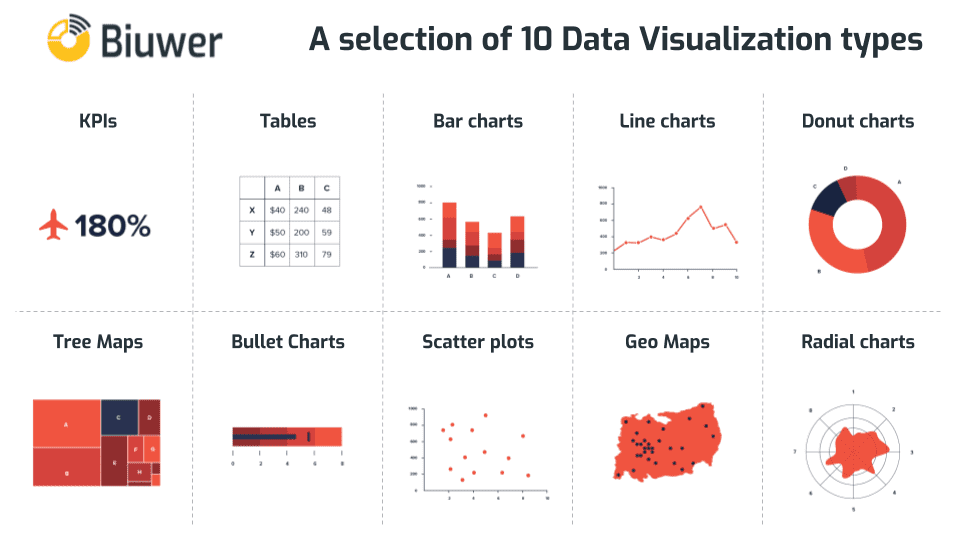
\includegraphics[width=1\textwidth]{content/img/Research/Visualisation/simple_visualisation_methods.png}
    \caption{Einfache Datenvisualisierungen in Form von Werten, Diagrammen, Tabellen und Karten \cite{morales2020picture}}
    \label{fig:einfacheDatenvisualisierung}
\end{figure}
\FloatBarrier

% paar Vor- Nachteile für verschiedene Diagramme

Die Visualisierungen in Abbildung \ref{fig:einfacheDatenvisualisierung} halten sich auch an wichtige Empfehlungen, um eine erfolgreiche Darstellung zu erstellen. Grafiken sollen laut Katy French nämlich eine vollkommene Geschichte erzählen. Dabei wird vor einer Überflut an Daten innerhalb der Visualisierung gewarnt, welche vom wesentlichen Grundgedanken der Darstellung ablenken würden. \cite{frenchsimplevis}

Ein weiterer Tipp bezieht sich auf die Auswahl einer bestimmten primären Farbe, welche mittels Helligkeit und Sättigung mehrere Farbtöne für das Diagramm erzeugt. Zusätzlich ist es immer sinnvoll, Beschriftungen leserlich zu gestalten, die Daten intuitiv zu ordnen und keine Elemente in Darstellungen einzufügen, welche zum Beispiel bei Präsentationen nur dazugesagt werden. \cite{frenchsimplevis}

Beim Designen eines Dashboards sind die Differenzen der verschiedenen Diagramme zu beachten. Denn nicht jedes Diagramm kann von Menschen mit der gleichen Effizienz interpretiert werden und einige Datensätze können in bestimmten Diagrammen nicht gut visualisiert werden. Balkendiagramme stellen Prozentwerte beispielsweise deutlich veranschaulicher dar, als Kreisdiagramme, da letztere die Bogenlänge als Maß für die Proportionalität nehmen. Nur durch richtige Anordnung der Kreissegmente können Benutzer die Daten richtig extrahieren. In Balkendiagrammen werden die Datensätze oft absteigend nach Proportionalität sortiert. \cite{2023diagrammarten}

Auch zwischen Säulen- und Balkendiagrammen gibt es Differenzen. Denn intuitiv befindet sich der Zeitfaktor in jedem Diagramm auf der x-Achse. Deswegen werden Vergleiche über einen gewissen Zeitraum immer mittels Säulendiagrammen dargestellt. Handelt es sich um einen längeren Zeitraum, dessen Gruppierungen die Anzahl 15 überschreiten, wird empfohlen, ein Liniendiagramm stattdessen zu wählen, da sonst zu viele Säulen vorhanden sind. Balkendiagramme eignen sich wiederum besonders für kategoriale Vergleiche, wie zum Beispiel verschiedene Genre bei Büchern und dessen Beliebtheit (Abbildung \ref{fig:GenreBuecherBeliebtheit}). Gruppierte Säulen- beziehungsweise Balkendiagramme sind immer dann zu wählen, wenn pro Zeiteinheit beziehungsweise Kategorie mehrere Datensätze bestehen. Falls diese Datensätze Mengen beschreiben, wie zum Beispiel Anzahl an Frauen und Männern - zusammengerechnet ergibt sich die Anzahl an Personen -, sind gestapelte Säulen- und Balkendiagramme eindeutig zu bevorzugen. In Darstellung \ref{fig:differentCharts} können Sie den Unterschied zwischen gruppierten und gestapelten Säulendiagrammen erkennen. \cite{marktler2020diagrammtypen}

\begin{figure}
    \centering
    \begin{subfigure}{.5\textwidth}
        \centering
        \includegraphics[width=0.9\linewidth]{content/img/Research/Visualisation/gruppiertes_Säulendiagramm.png}
        \caption{gruppiertes Säulendiagramm \cite{groupedChart}}
        \label{fig:groupedChart}
    \end{subfigure}%
    \begin{subfigure}{.5\textwidth}
        \centering
        \includegraphics[width=0.9\linewidth]{content/img/Research/Visualisation/gestapeltes_Säulendiagramm.png}
        \caption{gestapeltes Säulendiagramm \cite{stackedChart}}
        \label{fig:stackedChart}
    \end{subfigure}
    \caption{verschiedene Arten von Säulendiagrammen (auch bei Balkendiagrammen möglich)}
    \label{fig:differentCharts}
\end{figure}
\FloatBarrier

\begin{figure}
    \centering
    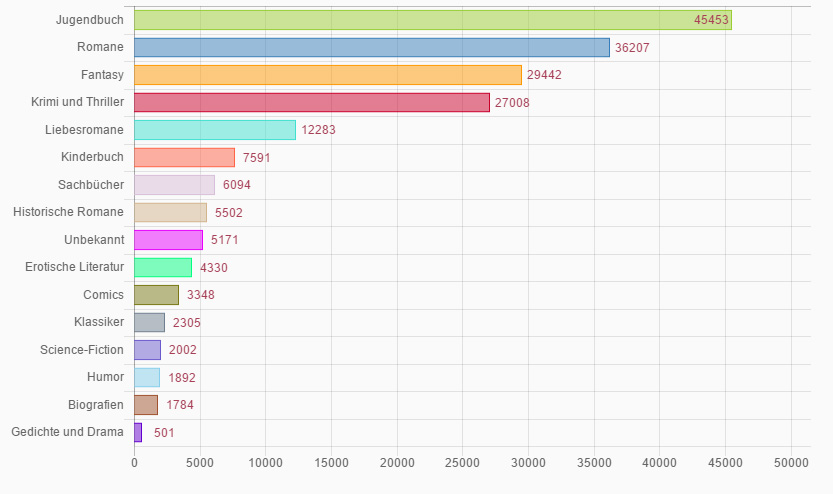
\includegraphics[width=1\textwidth]{content/img/Research/Visualisation/genres.jpg}
    \caption{Beliebtheit der verschiedenen Buchgenre im Jahr 2016 \cite{zeising2016genre}}
    \label{fig:GenreBuecherBeliebtheit}
\end{figure}
\FloatBarrier

Jede Diagrammart hat demnach ihre Daseinsberechtigung und soll auch für den spezifischen Anwendungsfall herangezogen werden. \cite{marktler2020diagrammtypen}

\subsection{Darstellung von komplexen Daten in Graphen, Heatmaps und Diagrammen}

Das Visualisieren von Daten allgemein - unabhängig von der Menge - unterstützt uns wesentlich bei Entscheidungen. Diese Hilfe bei der Findung relevanter Entscheidungen ist einer der essenziellsten Existenzgründe für Darstellungen im Allgemeinen. Die Herausforderung bei der grafischen Aufbereitung von stark vernetzten Daten liegt in der schieren Menge der Daten. Man spricht von \emph{Big Data}. \cite{2020simplevis,lin2023guide}

Pohan Lin erklärt in seinem Artikel die Schwierigkeit, große Datenmengen auf einfachen Bildschirmen intuitiv zu visualisieren, sodass Muster und Zusammenhänge erkannt und demenstprechend auch objektiv sinnvolle Schlüsse aus Daten gezogen werden können. Ebenso erläutert Eberhard Heins in einem Artikel von 2017 die Herausforderungen, welche mit der Visualisierung von Big Data kommen. Mit steigender Anzahl an Knoten und Kanten in einem Graphen wird dieser unübersichtlicher, da Muster in dem \wordindoublequotes{Farbteppich} nicht extrahiert werden können, was die Entscheidungshilfe signifikant reduziert. Ebenso leidet die Orientierung und Leserlichkeit der Darstellung darunter. Nur unter effizienter und übersichtlicher Umsetzung einer Big Data-Darstellung können die Vorteiler der Visualisierung genutzt werden. \cite{lin2023guide,heins2017herausforderungen}

Um ein ungefähres Bild von der schieren Menge an Informationen bei hoch korrelierenden Daten zu bekommen, wird Abbildung \ref{fig:BigData} hier kurz erläutert. Es handelt sich um eine Darstellung des sozialen Netzwerkes LinkedIn. In diesem Graphen hat jeder Konten die Bedeutung einer Person und jede Kante beschreibt eine Art von Beziehung zwischen den beiden anliegenden Personen. Die Extraktion hilfreicher Informationen kann bei Anbetracht dieser Grafik vergessen werden.

\begin{figure}
    \centering
    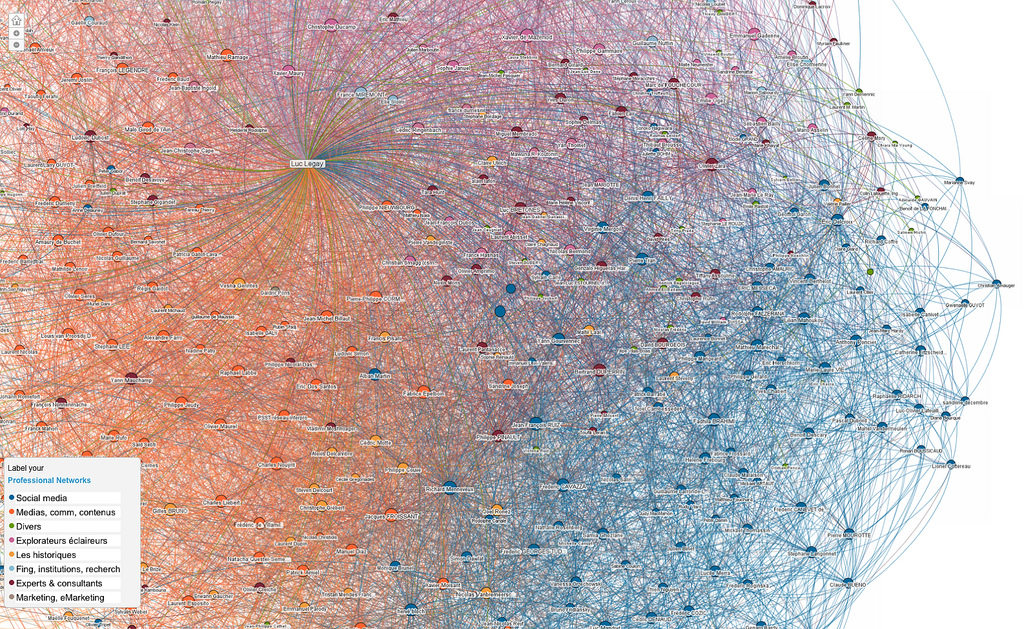
\includegraphics[width=1\textwidth]{content/img/Research/Visualisation/big_data_2.png}
    \caption{Stark vernetzte Daten in einem Graphen (LinkedIn Netzwerk) \cite{bigdata2014image}}
    \label{fig:BigData}
\end{figure}
\FloatBarrier

Die Komplexität eines Graphen kann mittels unterschiedlichen Ansätzen reduziert werden. Logischerweise führt eine Reduktion der Datenmenge automatisch zu einer übersichtlicheren Visualisierung und infolgedessen zu einer besseren Orientierung und Leserlichkeit beziehungsweise Erkennbarkeit. Jedoch kommt die Reduktion mit dem großen Nachteil des Informationsverlustes. Ein weiterer Ansatz definiert aggregierte Visualisierungstechniken als Zusammenfassung gewisser Informationen (\emph{Clustering}). Im Folgenden werden verschiedene Darstellungsmethoden im Detail analysiert. \cite{heins2017herausforderungen}

\subsubsection{Vereinfachung der komplexen Daten mittels Clustering}

Graph-Clustering ist eine Methode zur Vereinfachung eines komplexen Graphen, indem Gruppierungen, Muster, Zusammenhänge oder Strukturen mittels Algorithmen extrahiert werden. Diese neuen Daten sind entscheidend für Datenwissenschaftler. Denn aus den Erkenntnissen dieser können fundierte Entscheidungen in verschiedenen Bereichen, wie zum Beispiel Marketing, Bioinformatik oder auch die Entdeckung von Fehlern oder Sicherheitslücken innerhalb eines Netzwerkes, getroffen werden. \cite{pusic2023clustering}

Die Algorithmen hinter Graph-Clustering sind unterstützt von maschinellem Lernen. Die künstliche Intelligenz versucht hierbei Gemeinsamkeiten der einzelnen Nodes innerhalb des Graphes zu finden. Diese Ähnlichkeiten können entweder direkte Eigenschaften der Knoten sein oder Berechnungen aufgrund der Konnektivität zwischen den Knoten im Graphen. In Abbildung \ref{fig:GraphClusteringAlgorithm} kann auf der rechten Seite die Gruppierung der Knoten des Ausgangsgraphen (links) mittels farblichen Markierungen festgestellt werden. \cite{pusic2023clustering}

\begin{figure}
    \centering
    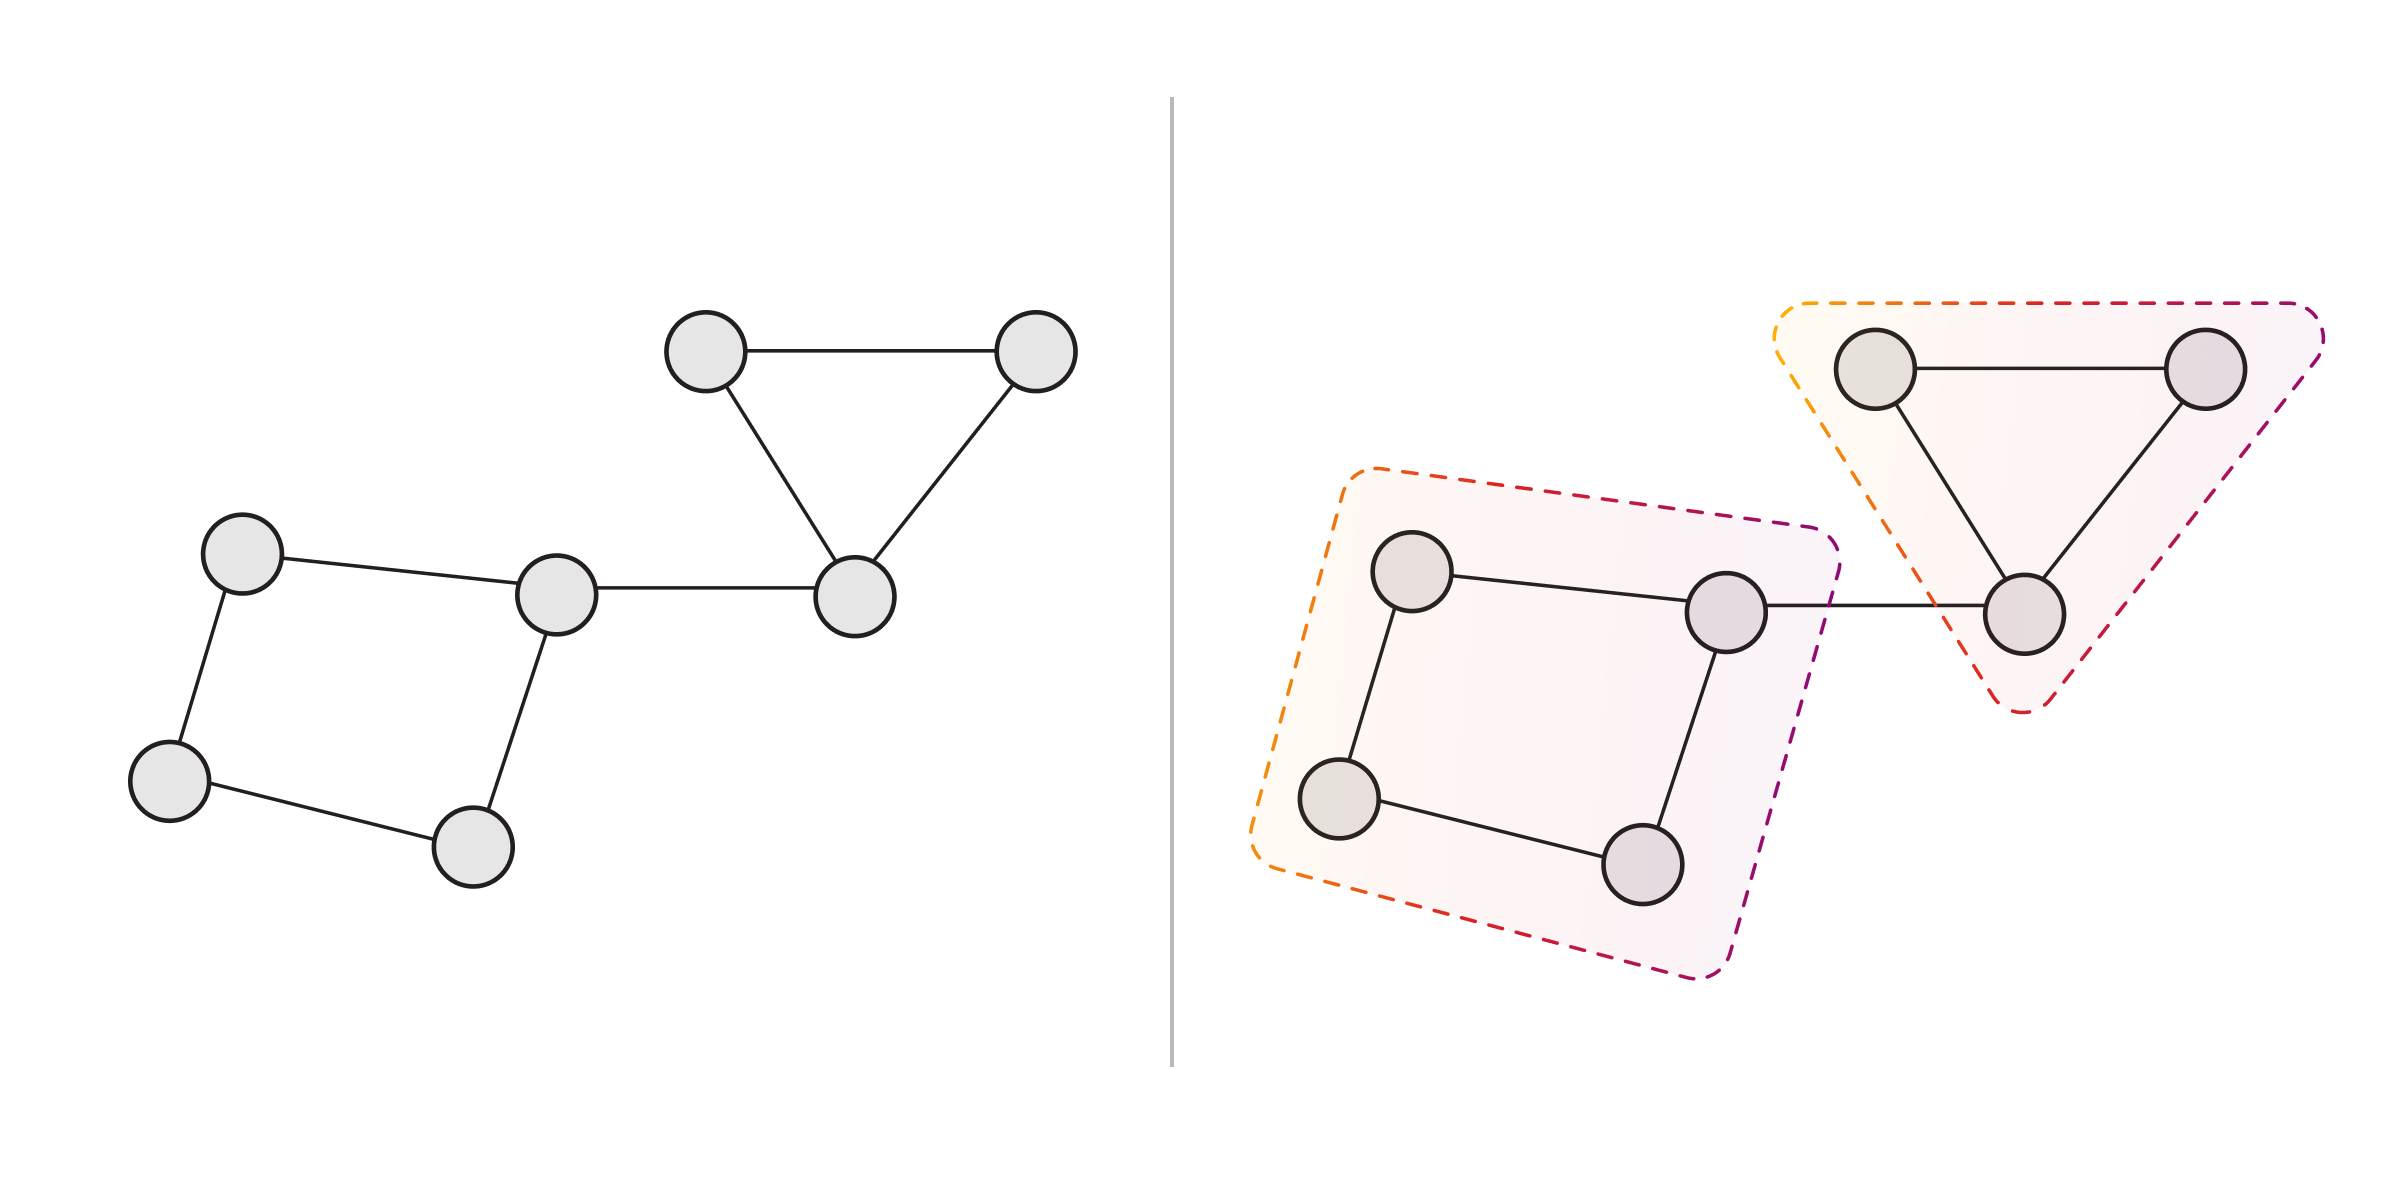
\includegraphics[width=1\textwidth]{content/img/Research/Visualisation/graph_clustering_algorithm.png}
    \caption{Clustering eines Graphen \cite{pusic2023clustering}}
    \label{fig:GraphClusteringAlgorithm}
\end{figure}
\FloatBarrier

Das Clustering eines Graphen kann auch nur auf irrelevante Daten angewandt werden, welche jedoch gruppiert in der Visualisierung beibehalten werden sollen. Beispielsweise können aktuelle Daten in der Mitte möglichst detailliert aufbereitet sein, während Daten aus vergangenen und demnach veralteten Jahre rundherum aggregiert dargestellt sind. \cite{heins2017herausforderungen}

\subsubsection{Vereinfachung der verknüpften Daten mittels farblichen Abstufungen}

Solange die Zugänglichkeit einer Grafik auch für Menschen mit Farbsehschwächen gegeben ist, sind Farben ein wunderbarer Weg, um verschiedene Daten in Diagrammen oder auch Grids zu visualisieren. Sogenannte \emph{Heatmaps} eignen sich besonders gut, um eine große Datenmenge geordnet und gruppiert darzustellen. Dabei werden die Daten in einem Diagramm mit zwei Achsen farblich auf Rechtecken dargestellt, wobei die Farbe Auskunft über die Intensität in der jeweiligen Zeile und Spalte gibt. Empfohlen wird eine Verwendung einer Legende, um die Bedeutung der Farben in der Heatmap zu erklären. \cite{yiheatmap,cinar2023heatmap,kassamara2020heatmap}

Beispielsweise können Sie aus der Abbildung \ref{fig:HeatmapGitHub} deutlich ablesen, dass der Benutzer fast ausschließlich an Wochentagen arbeitet. Samstage und Sonntage sind nämlich in den meisten Fällen grau, was laut Legende bedeutet, dass keine Contributions von diesem Benutzer an diesen Tagen gemacht worden sind. Und genau solche Informationen sind in vielen anderen Bereichen entscheidend für Datenwissenschaftler.

\begin{figure}
    \centering
    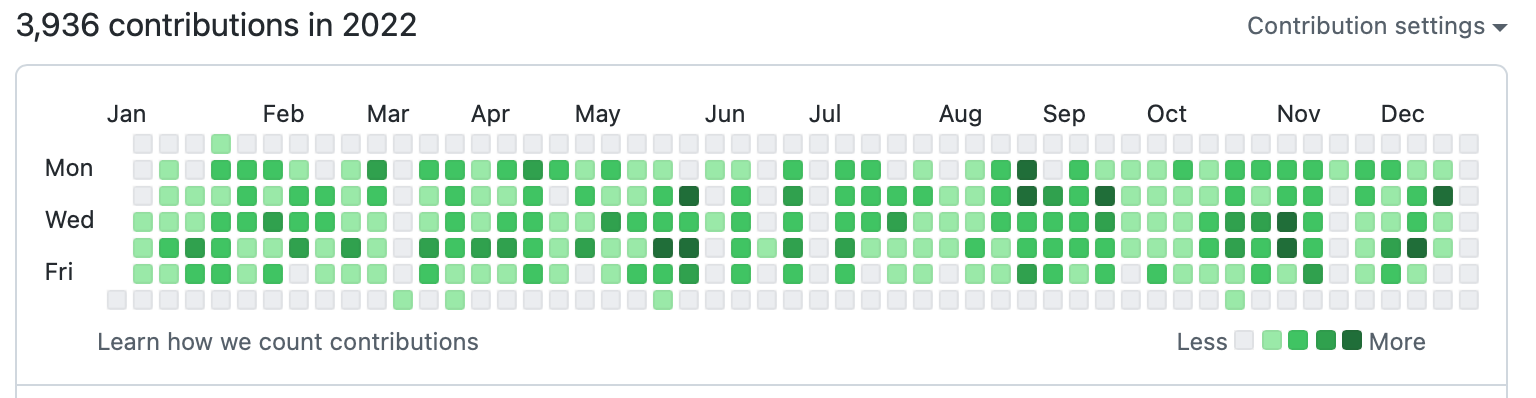
\includegraphics[width=1\textwidth]{content/img/Research/Visualisation/heatmap.png}
    \caption{Heatmap der Beiträge eines GitHub Benutzers im Jahr 2022 \cite{yiheatmap}}
    \label{fig:HeatmapGitHub}
\end{figure}
\FloatBarrier

\subsubsection{Vereinfachung der vernetzten Daten mittels Interaktivität}

Die Visualisierung von Graphen inkludiert meistens eine Zoom- und Filterfunktionalität. Neben diesen Orientierungshilfen gibt es auch die Möglichkeit, Daten in Diagrammen und Graphen mittels Lupentechniken zu vereinfachen. Dabei werden gewisse Daten mittels Verzerrungen hervorgehoben und die restlichen Daten nur verkleinert am Rande angezeigt. Das explorative Verhalten der Visualisierung wird umso mehr verbessert, wenn die Lupenfunktionalität mit dem Benutzer interagiert. Eine besonders intuitive Interaktionsmöglichkeit ist die Lupenverfolgung des Mauszeigers. In anderen Worten kann der Benutzer die Position der Lupe in der Grafik mittels Maus direkt beeinflussen. \cite{bostock2012fisheye}

In Abbildung \ref{fig:LupentechnikGridFisheye} kann das Prinzip der Lupe auf einem Grid gut erkannt werden. Die Verzerrungsmethode heißt hierbei \emph{Fisheye}.

\begin{figure}
    \centering
    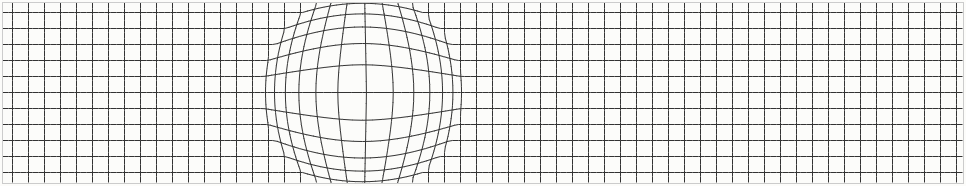
\includegraphics[width=1\textwidth]{content/img/Research/Visualisation/distortion_fisheye.png}
    \caption{Demonstration der Lupentechnik Fisheye auf einem Grid \cite{bostock2012fisheye}}
    \label{fig:LupentechnikGridFisheye}
\end{figure}
\FloatBarrier

Auch, wenn ein statisches Bild den Effekt eines Fischauges in einem Graphen nicht perfekt veranschaulichen kann, sehen Sie in Abbildung \ref{fig:FisheyeGraph} einen Graphen, dessen Knotenpunkt \wordindoublequotes{Brujon} momentan mittels Lupe analysiert wird.

\begin{figure}
    \centering
    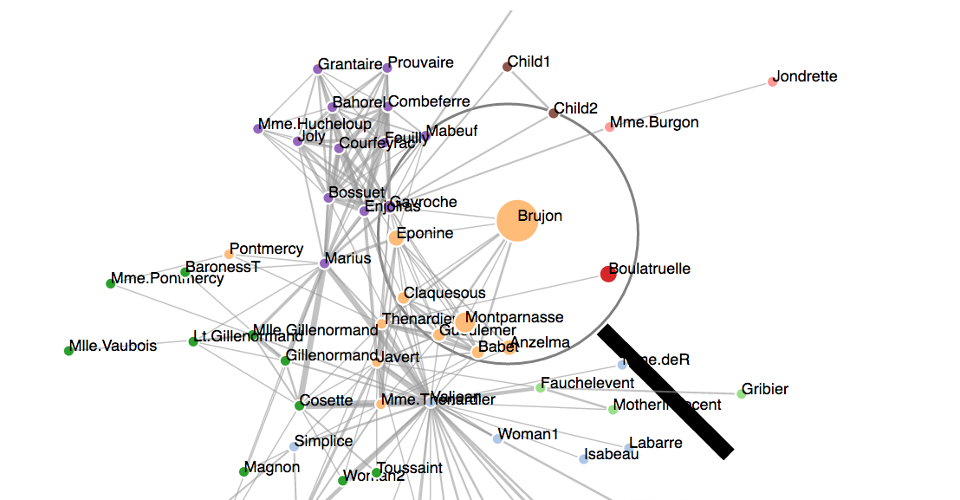
\includegraphics[width=1\textwidth]{content/img/Research/Visualisation/fisheye_graph.png}
    \caption{Demonstration des Fischauges in einem Graphen \cite{githubgistFisheye}}
    \label{fig:FisheyeGraph}
\end{figure}
\FloatBarrier

Die Lupentechnik muss nicht immer mit dem Fisheye-Effekt visualisiert sein. Es gibt zum Beispiel auch die Möglichkeit, eine \emph{kartesische Verzerrung} (Abbildung \ref{fig:LupentechnikGridCartesian}) interaktiv zu verwenden. Dabei werden die Skalierungen der Achsen je nach Mausposition so angepasst, dass es sich so anfühlt, als wäre der Inhalt darunter am nähesten beziehungsweise größten. \cite{bostock2012fisheye}

\begin{figure}
    \centering
    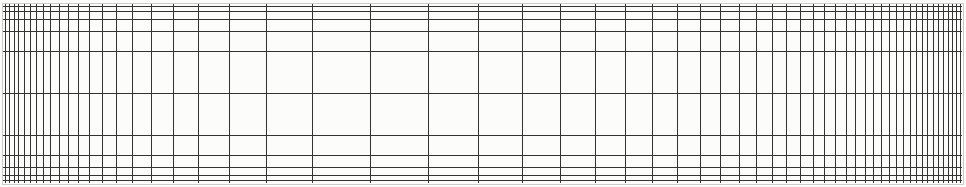
\includegraphics[width=1\textwidth]{content/img/Research/Visualisation/distortion_cartesian.png}
    \caption{Demonstration der kartesischen Verzerrungstechnik auf einem Grid \cite{bostock2012fisheye}}
    \label{fig:LupentechnikGridCartesian}
\end{figure}
\FloatBarrier

\subsubsection{Vereinfachung der vielschichtigen Daten mittels Reduktion}

Die wohl einfachste Methode, stark vernetzte Daten intuitiv und verständlich darzustellen, ist das Entfernen gewisser Datensätze beziehungsweise gewisse Attribute oder Dimensionen von Datensätzen aus der Grafik durch spezifische Filterung der Daten. Dadurch werden nur die wichtigsten Daten angezeigt und der Benutzer kann diese interpretieren und somit vernünftige Entscheidungen daraus schließen. Die Reduktion der Daten hat jedoch den Nachteil, dass einige, eventuell essenzielle Informationen verloren gehen. Bestimmte Zusammenhänge und Strukturen der Daten können nämlich nicht extrahiert werden, wie es jedoch bei anderen Visualisierungsmöglichkeiten (wie zum Beispiel Clustering) der Fall ist. Dieser unvermeidliche Informationsverlust sollte bei der Reduktion minimiert werden, um in Bezug auf Richtigkeit möglichst nahe an den ungefilterten Daten zu bleiben. \cite{heins2017herausforderungen,beilhammer2017interpretation}

\subsubsection{Darstellung der vereinfachten Daten durch Mischformen}

\wordindoublequotes{Best practice}-Visualisierungen vermischen verschiedene Formen der Vereinfachung und erstellen Grafiken, welche die wesentlichsten Informationen kurz und knapp auf den Punkt darstellen. Beispielsweise hat Google in der Dokumentation von Google Maps eine geobasierte Heatmap\footnote{Hierbei wird der Begriff \wordindoublequotes{Heatmap} allgemein verwendet, da diese nicht an ein Raster gebunden ist.} herangezogen, welche in Abbildung \ref{fig:GoogleMapsHeatmap} zu Demonstrationszwecken abgebildet ist.

\begin{figure}
    \centering
    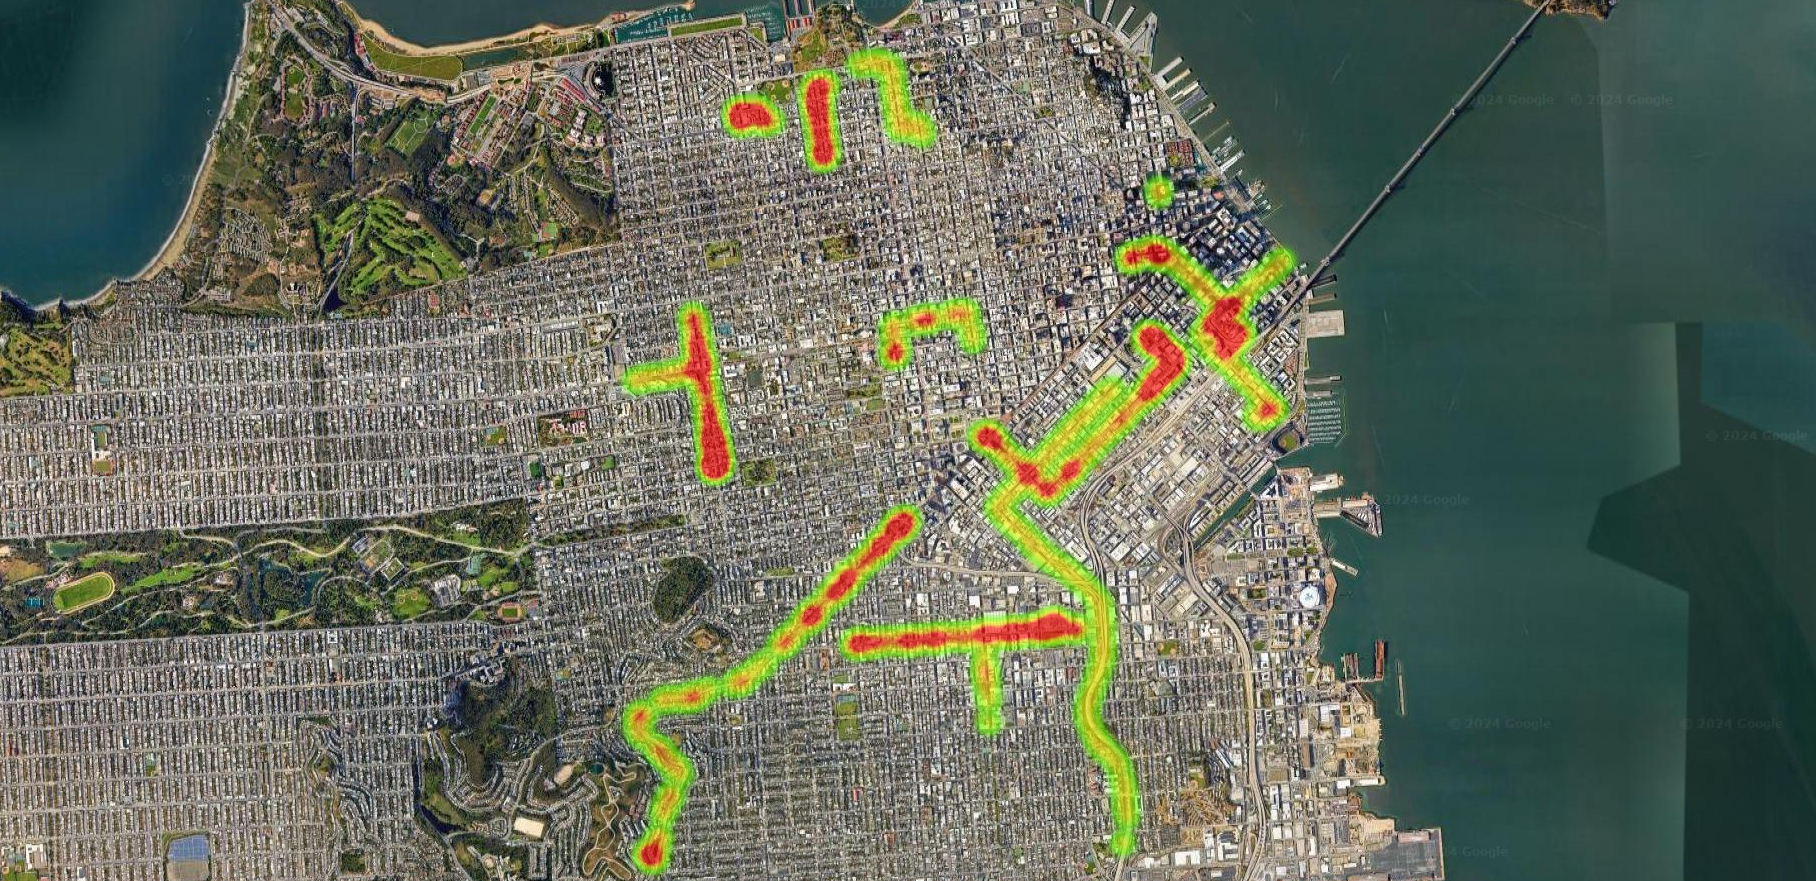
\includegraphics[width=1\textwidth]{content/img/Research/Visualisation/Google_Maps_Heatmap.png}
    \caption{Exemplarische geobasierte Heatmap aus der Google Maps Dokumentation}
    \label{fig:GoogleMapsHeatmap}
\end{figure}
\FloatBarrier